\section{\large{\textbf{Junkers Ju 87}}}
%========================

\subsection{Początki}


\begin{frame}{\Huge{\textbf{Ju 87 - Początki}}}
	\begin{columns}[t]
		\column{0.525\textwidth} 
			\justifying
			
Jednym z najważniejszych osiągnięć niemieckiego lotnictwa był bombowiec nurkujący \textbf{Junkers Ju 87}, znany jako Stuka. Choć inne państwa również korzystały z bombowców nurkujących, to Niemcy używali Stuki w sposób nieporównywalny, przez długi czas i z dużym powodzeniem. Samolot ten zadebiutował podczas hiszpańskiej wojny domowej i odegrał kluczową rolę w kampaniach Wehrmachtu w Polsce i Francji, a także podczas walk w Norwegii. \\
W styczniu 1925 roku Hugo Junkers, wspólnie z braćmi Flormanami, założył firmę AB Flygindustri w Szwecji, aby obejść postanowienia traktatowe ograniczające produkcję zbrojeniową. Tam powstał obiecujący samolot myśliwski K 47. \\
W 1929 roku metalowy jednopłat po raz pierwszy wzbił się w powietrze, osiągając prędkość bliską 300 km/h, ale z powodu braku funduszy niemieckich sił zbrojnych tylko cztery z czternastu wyprodukowanych samolotów były używane jako maszyny quasi-cywilne.

		\column{0.5\textwidth}
			\begin{figure}
				\centering
				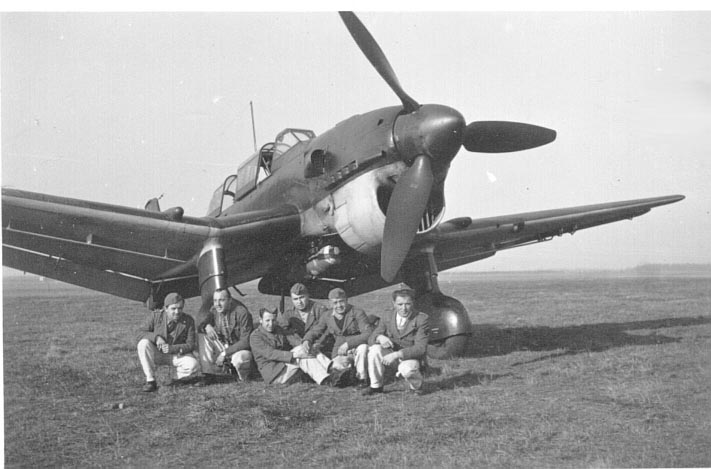
\includegraphics[scale=1.9]{images/ju87-01.jpg}	
				\caption{\textit{Ju 87 ''Stuka''}}
			\end{figure}
	\end{columns}
\end{frame}


%~~~~~~~~~~~~~~~~~~~~~~~~~~~~~~~~~

\subsection{Ernst Udet}


\begin{frame}{\Huge{\textbf{Ju 87 - Ernst Udet}}}
	\begin{columns}[t]
		\column{0.6\textwidth} 
			\justifying
			
Kluczową postacią w promowaniu bombowców nurkujących był \textbf{Ernst Udet}, który po obejrzeniu pokazów w USA namówił niemiecki rząd do zakupu maszyn, co finalnie doprowadziło do zakupu dwóch samolotów Curtiss Hawk. W 1934 roku Biuro Techniczne RLM ogłosiło wymagania dotyczące bombowca nurkującego, a projekt Henschel Hs 123 zajął pierwsze miejsce. Mimo że był to samolot przejściowy, Hs 123 służył jako szturmowiec do 1944 roku. RLM zwróciło uwagę na Junkersa, który pracował nad Ju 87, prototypie bombowca nurkującego. Po kilku poprawkach konstrukcyjnych, takich jak zmiana usterzenia i dodanie hamulców aerodynamicznych, Ju 87 rozpoczął próby w 1936 roku. \\
W marcu 1936 roku odbyły się porównawcze testy różnych konstrukcji, w których Ju 87, dzięki swojej pionowej trajektorii bombardowania, wykazał się znacznie lepszą celnością niż konkurenci. Ostateczne zwycięstwo Junkersa potwierdził Ernst Udet, który miał groźny wypadek podczas lotu próbnego.

		\column{0.4\textwidth}
			\begin{figure}
				\centering
				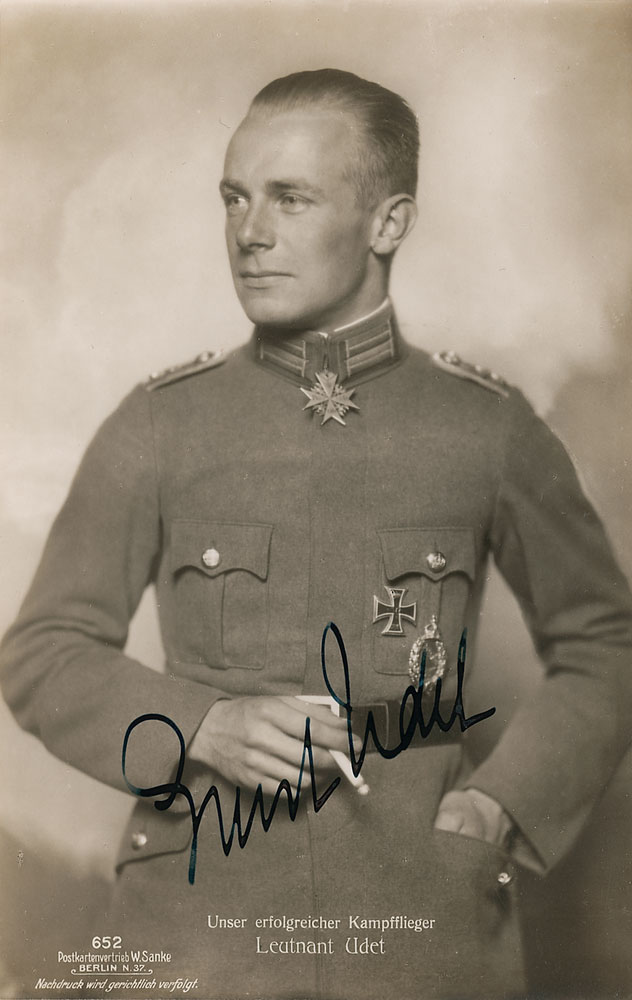
\includegraphics[scale=0.18]{images/ju87-02.jpg}
				\caption{\textit{Ernst Udet}}
			\end{figure}
	\end{columns}
\end{frame}


%~~~~~~~~~~~~~~~~~~~~~~~~~~~~~~~~~

\subsection{Warianty}


\begin{frame}[t]{\Huge{\textbf{Ju 87 - Warianty}}}
	\begin{columns}[t]
		\column{0.5\textwidth} 

{\large{\textbf{Wariant A – Anton}}	}\\~\
	\justifying

W 1936 roku powstał prototyp V-4, który wprowadził powiększony statecznik pionowy. Na jego podstawie stworzono serię przedprodukcyjną A-0, a następnie pierwszą produkcyjną A-1. Samoloty A-1 były napędzane silnikiem Jumo 210 Ca o mocy 630 KM, uzbrojone w dwa karabiny maszynowe: jeden MG-17 w prawym skrzydle i ruchomy MG-15 obsługiwany przez obserwatora. Mogły przenosić jedną bombę o wadze 250 kg lub do 500 kg, kosztem obecności tylnego strzelca. Pilot miał do dyspozycji celownik optyczny i system automatycznego wyprowadzania z nurkowania. Pierwsze egzemplarze Ju 87A-1 trafiły do Luftwaffe na początku 1937 roku, a produkcję wersji A zakończono przed wybuchem wojny.

		\column{0.5\textwidth}

{\large{\textbf{Wariant B – Bertha}}	}\\~\
	\justifying
	
Wersja Ju 87B-1 wprowadzała znaczące zmiany, w tym mocniejszy silnik Jumo 211 A (1100 KM) i nową konstrukcję podwozia. Osłona kabiny zmieniła się na przesuwaną, a w podwoziu zainstalowano syreny, które uruchamiały się w locie nurkowym, co miało siać panikę wśród przeciwników. Wersja B-2, produkowana od 1939 roku, miała jeszcze mocniejszy silnik (Jumo 211 Da, 1200 KM) oraz zmodyfikowane uzbrojenie, które mogło obejmować jedną bombę ćwierćtonową pod kadłubem lub dwie mniejsze pod skrzydłami. Wersja B-2 zakończyła produkcję w 1941 roku z łączną liczbą 1634 egzemplarzy. 

	\end{columns}
\end{frame}

%----------------------------------------------

\begin{frame}[t]{\Huge{\textbf{Ju 87 - Warianty}}}
	\begin{columns}[t]
		\column{0.5\textwidth} 

{\large{\textbf{Wariant C – Caesar}}}	\\~\
	\justifying

Wczesna wersja C, zaprojektowana w 1939 roku, miała służyć jako samolot pokładowy dla lotniskowca Graf Zeppelin. Zmniejszono rozpiętość skrzydeł, wprowadzono składane skrzydła i systemy umożliwiające start z katapulty. Samolot był wyposażony w ogrzewanie kabiny i nadmuchiwaną łódkę ratunkową, a także zwiększono pojemność zbiorników paliwa do 2500 litrów.

		\column{0.5\textwidth}
		
{\large{\textbf{Wariant D – Dora}}}	\\~\
	\justifying

Model Ju 87 D-1 miał być początkowo wyposażony w silnik Daimler-Benz DB 603, jednak okazał się on gorszy niż Jumo 211, więc zrezygnowano z niego. W serii D ulepszono system chłodzenia, poprawiono aerodynamikę kadłuba oraz powiększono kabinę. Dodatkowo wzmocniono siłę ognia, instalując karabin MG 81Z kalibru 7,92 mm, a nowe silniki Jumo 211 J-1 i Jumo 211 P dostarczały odpowiednio 1420 i 1500 KM. Zwiększono także pojemność zbiorników paliwa do 1370 litrów, umożliwiając loty o czasie do 4 godzin z dodatkowymi zbiornikami.

	\end{columns}
\end{frame}

%----------------------------------------------

\begin{frame}[t]{\Huge{\textbf{Ju 87 - Warianty}}}
	\begin{columns}[t]
		\column{0.5\textwidth} 

{\large{\textbf{Wariant G – Gustav}}}	\\~\
	\justifying
	
Oparta na modelu D, była przeznaczona do niszczenia czołgów i stanowiła ostatnią masowo produkowaną wersję Ju 87, wykorzystywaną na froncie wschodnim. Po utracie przewagi Wehrmachtu nad Armią Czerwoną, Junkers przystosował Ju 87 do zwalczania sił pancernych. W odpowiedzi na żądania Luftwaffe o nowy samolot do walki z czołgami, w grudniu 1942 roku przeprowadzono testy Ju 87 D z działkami przeciwpancernymi, tworząc wersję Gustav. Model G-1 bazował na wersji D-3, a G-2 na D-5 z dłuższymi skrzydłami. Obie wersje uzbrojono w działka Bordkanone BK 3,7 mm i opancerzenie podobne do radzieckiego Ił-2, chroniące załogę podczas ataków z niskiego pułapu.

		\column{0.5\textwidth}
		
{\large{\textbf{Wariant R – Richard}}}	\\~\
	\justifying
	
Na początku 1940 roku, niektóre egzemplarze wersji B-1 i B-2 przekształcono w bombowce dalekiego zasięgu (wersja R). Zwiększono pojemność zbiorników paliwa, co ograniczyło możliwości ładunkowe do jednej bomby 25 kilogramowej. W modelu R-2 po raz pierwszy zastosowano system identyfikacji swój-obcy (IFF), co miało na celu poprawę bezpieczeństwa operacji powietrznych.

	\end{columns}
\end{frame}